\documentclass[paperheight=140cm,paperwidth=100cm,portrait]{./baposter}

% intro, system, construction, Electronics and software, - Flowchart, Results, Acknowledgement
% todo:
% bigger title
% caption darkblue


\usepackage{wrapfig}
\usepackage{lmodern}


\usepackage[paperheight=89.5cm,paperwidth=128cm,margin=2cm,heightrounded,showframe]{geometry}

\usepackage[utf8]{inputenc} %unicode support
\usepackage[T1]{fontenc}
\usepackage{amsmath}
\usepackage[font=small,labelfont=bf]{subcaption} % <-- changed to subcaption
\usepackage{graphicx}
\usepackage{xcolor}
\usepackage{tikz}
\usepackage{blindtext}
\usetikzlibrary{shapes.geometric, arrows}
\usetikzlibrary{decorations.markings}
\usetikzlibrary{decorations.pathmorphing,patterns}


\tikzstyle directed=[postaction={decorate,decoration={markings, % arrows on the field lines
mark=at position .1 with {\arrowreversed[scale=1.5]{stealth}},
mark=at position .9 with {\arrowreversed[scale=1.5]{stealth}}}}]
\tikzstyle tangent=[postaction={decorate,decoration={markings, % Tangent to the field line
mark=at position .7 with {\draw[ultra thick,stealth-,green!60!black,solid](-12pt,0)--(12pt,0)node[above]{$\vec{B}$};}}}]
\tikzstyle fLines=[thick,dashed,directed,tangent]
% tikz stuff for the flow charts
\tikzstyle{startstop} = [rectangle, rounded corners, minimum width=3cm, minimum height=1cm,text centered, draw=black, fill=red!30]
\tikzstyle{io} = [trapezium, trapezium left angle=70, trapezium right angle=110, minimum width=1cm, minimum height=1cm, text centered, draw=black, fill=blue!30]
\tikzstyle{process} = [rectangle, minimum width=3cm, minimum height=1cm, text centered, draw=black, fill=orange!30]
\tikzstyle{decision} = [diamond, minimum width=3cm, minimum height=1cm, text centered, draw=black, fill=green!30]
\tikzstyle{arrow} = [thick,->,>=stealth]

% #1 number of teeth
% #2 radius intern
% #3 radius extern
% #4 angle from start to end of the first arc
% #5 angle to decale the second arc from the first
\newcommand{\gear}[5]{%
    \foreach \i in {1,...,#1} {%
        [rotate=(\i-1)*360/#1]
        (0:#2) arc (0:#4:#2)
        [rounded corners=1.5pt]
        -- (#4+#5:#3)
        arc (#4+#5:360/#1-#5:#3)
        -- (360/#1:#2)
    }
}


\selectcolormodel{cmyk}

\graphicspath{{figures/}} % Directory in which figures are stored


\newcommand{\compresslist}{%
    \setlength{\itemsep}{0pt}%
    \setlength{\parskip}{1pt}%
    \setlength{\parsep}{0pt}%
}

\newenvironment{boenumerate}
{\begin{enumerate}
     \renewcommand\labelenumi{\textbf\theenumi.}}
     {
\end{enumerate}}



\begin{document}


    \definecolor{darkgreen}{cmyk}{0.8,0,0.8,0.45}
    \definecolor{lightgreen}{cmyk}{0.8,0,0.8,0.25}
    \definecolor{hopro_blue}{HTML}{62C3EB}
    \definecolor{hopro_darkblue}{HTML}{
25334D
}

    \begin{poster}
    {
        grid=false,
        headerborder=open, % Adds a border around the header of content boxes
        colspacing=1.3em, % Column spacing
        rowspacing=1.3em, % Row spacing
        bgColorOne=white, % Background color for the gradient on the left side of the poster
        bgColorTwo=white, % Background color for the gradient on the right side of the poster
        borderColor=hopro_blue, % Border color
        headerColorOne=hopro_blue, % Background color for the header in the content boxes (left side)
        headerColorTwo=hopro_blue, % Background color for the header in the content boxes (right side)
        headerFontColor=white, % Text color for the header text in the content boxes
        boxColorOne=white, % Background color of the content boxes
        textborder=rounded, %rectangle, % Format of the border around content boxes, can be: none, bars, coils, triangles, rectangle, rounded, roundedsmall, roundedright or faded
        eyecatcher=false, % Set to false for ignoring the left logo in the title and move the title left
        headerheight=0.15\textheight, % Height of the header
        headershape=rounded, % Specify the rounded corner in the content box headers, can be: rectangle, small-rounded, roundedright, roundedleft or rounded
        headershade=plain,
        boxheaderheight=0.95cm,
        headerfont=\huge\textsf, % Large, bold and sans serif font in the headers of content boxes
%textfont={\setlength{\parindent}{1.5em}}, % Uncomment for paragraph indentation
        linewidth=2pt % Width of the border lines around content boxes
%        set font size in the content boxes
    }
    {}
%
%----------------------------------------------------------------------------------------
%   TITLE AND AUTHOR NAME
%----------------------------------------------------------------------------------------
%
    {

        \noindent
        \begin{minipage}{.1\linewidth}
            
\includegraphics[width=3.5cm]{../../photos/hopro_logo}
        \end{minipage}%
        \begin{minipage}{.05\linewidth}
        \end{minipage}
        \begin{minipage}{.9\linewidth}
            \centering
            \textsf{
                \fontsize{30}{8}\selectfont
                Designing, assembling \& programming \\a foosball goalkeeper robot
            }\\
            \sf\vspace{0.5em}
            \fontsize{18}{8}\selectfont
            Jan Wilhelm, 6e \hspace{0.3cm} \textbf{Supervisor}: Clemens Pohle, \textbf{Advisor:} Dr. Hugo Leonel Cabrera Cifuentes\\ \vspace{0.5cm} \selectfont Kantonsschule Hohe Promenande Zürich, Schuljahr 2024/2025
        \end{minipage}
        \vspace{1cm}

%        \textsf %Sans Serif
%        {DeCAF -- Discrimination, Comparison, Alignment algorithm for small molecules.
%        }
    } % Poster title
%    {\vspace{1em} Marta Stepniewska, Pawel Siedlecki\\ % Author names
%    {\small \vspace{0.7em} Department of Bioinformatics, Institute of Biochemistry and Biophysics, PAS, Warsaw, Pawinskiego 5a}} % Author email addresses
    {
%        \sf\vspace{0.5em}\\
%        Marta Stepniewska* and Pawel Siedlecki
%        \vspace{0.1em}\\
%        \small{Department of Bioinformatics, Institute of Biochemistry and Biophysics, PAS, Pawinskiego 5a, 02-106 Warsaw, Poland
%        \vspace{0.2em}\\
%        martasd@ibb.waw.pl}
    }

        \headerbox{1. Introduction}{name=introduction,column=0,row=-0.04, span=3}{

%Whether a machine can surpass a human in a specific task has fascinated people since the first machines
%were created. Over time, machines have outperformed humans in many areas, from simple calculations
%to complex strategy games like chess. With advancements in AI, machines are now capable of tasks like
%driving cars. But can a machine beat a human in a game of foosball (table soccer)? Unlike chess,
            Foosball (table soccer) is fast-paced and unpredictable, requiring quick reflexes and real-time decision-making.
            This makes it a perfect
            challenge for testing the limits of AI and robotics.
            The \textbf{goal of this project} is to \textbf{build a foosball-playing
            machine that can play with a human}. The machine will rely on a camera to monitor the game from below
            and will be controlled by a computer using two motors per axis to move the players and shoot the ball.
            The goal is to build and
            test a foosball goalkeeper robot as a proof of concept, that a machine could compete with a human player.

        }


        \headerbox{2. Robot set-up}{name=model,column=0,below=introduction,span=1}{

            \setcaptiontype{figure}% Fake a figure environment

            A simple diagramm of the final system is shown below.
            The system consists of a camera below the table, to monitor the game.
            The camera is connected to a PC, which processes the images and sends the commands to the controller unit.
            The controller unit moves the motors to the desired position.
%            \begin{figure}[h]
%                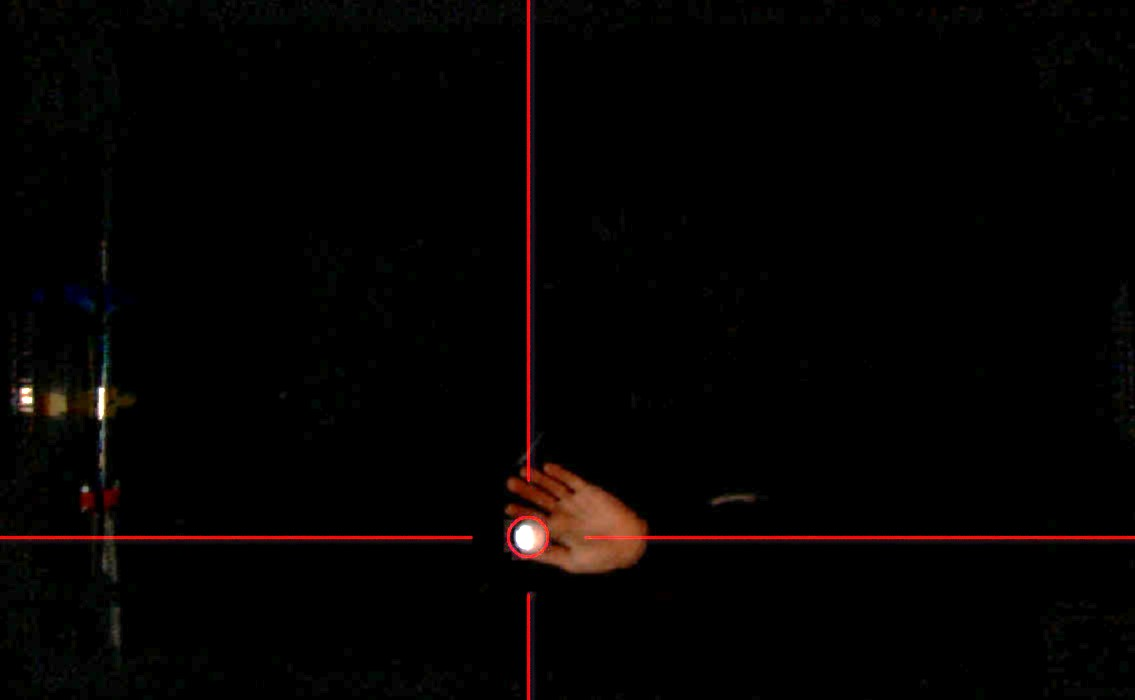
\includegraphics[width=\linewidth]{../../photos/ball_detection}
%            \end{figure}
            \begin{center}
%            \begin{figure}[h]
                \centering
                \scalebox{0.48}{
                    \begin{tikzpicture}
                        \draw[fill=green!5] (7, 10) rectangle (0, 0);
                        \begin{scope}
                            [shift={(3.5, 0)}]
                            \node[below] {Foosball table};
                        \end{scope}
%%        draw a circle in the middle and an arrow pointing there labling it the camera
                        \draw[fill=blue!30] (3.5, 5) circle (0.5) node[below, yshift=-0.5cm] {Camera below table};
%%        \draw[<-] (4.1, 5) -- (8, 5) node[above] {Camera};
%%            pc
                        \draw[fill=orange!30] (10, 9) rectangle (12, 11) node[pos=0.5] {PC};
%%            cable from camera to pc
                        \draw[->, blue] (3.5, 5.5) -- (3.5, 6) -- (11, 6) -- (11, 8.8);
%            controler (Arduino)
                        \draw[fill=orange!30] (6, 10) rectangle (9, 11) node[pos=.5]{Controller unit};
                        \draw[->, blue] (10, 10.5) -- (9.2, 10.5);
%%            move motor
                        \draw[fill=blue!30] (7, 6.5) rectangle (8.5, 8) node[pos=.5,
                        text width=1.5cm,align=center
                        ] {Move motor};
                        \begin{scope}
                            [shift={(7.75, 7.25)}, scale=0.4]
                            \draw \gear{18}{2}{2.4}{10}{2};
                        \end{scope}
                        \draw[fill, black] (7.75, 7.25) circle (0.03);
                        \draw[<-, blue](7.75, 8.2) -- (7.75, 10);
%        tube
                        \draw[fill=black!20] (0, 8.75) rectangle (9, 8.25) node[pos=.5, shift={(1, 0)}] {Tube};
                        \draw[fill=blue!30] (0, 9.25) rectangle (-1, 7.75) node[midway, left, shift={(-.5, 0)}] {Shoot motor};
                        \draw[->, blue] (6, 10.5) -- (-0.5, 10.5) -- (-0.5, 9.45);
                        \draw[fill=red] (3.5, 8.5) circle (0.5) node[below, yshift=-0.5cm] {Goalkeeper};
                    \end{tikzpicture}
                }
                \caption*{\color{hopro_darkblue}The foosball robot system}
                \label{fig:system}
%            \end{figure}

            \end{center}
        }


        \headerbox{4. Software \& Electronics}{name=electronics,column=0,below=model,span=1}{
            The software detects the ball on the table and predicts the future position and then the electronics give the correct commands to the motors.
            \begin{center}
                \setcaptiontype{figure}% Fake a figure environment
                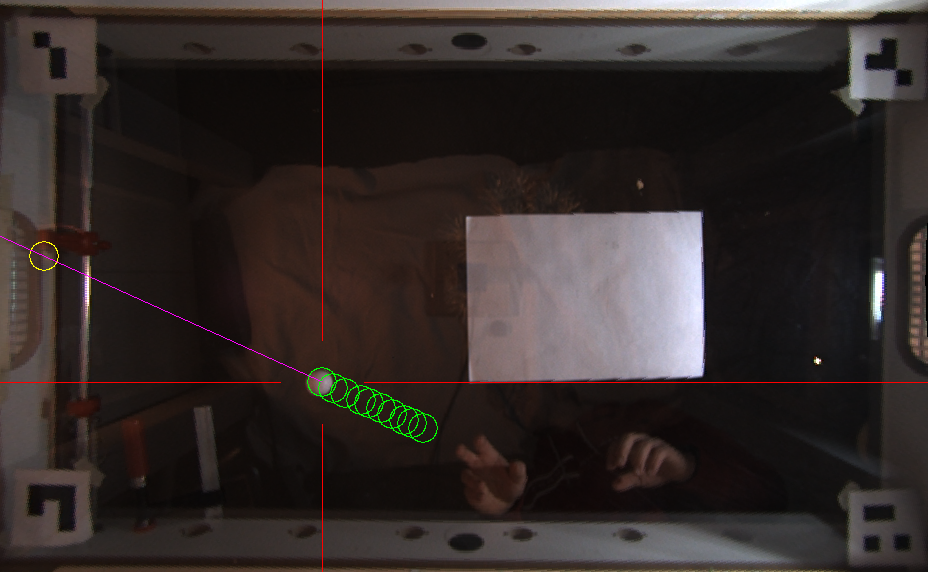
\includegraphics[width=\linewidth]{../../photos/ball_prediction2}
                \caption*{\color{hopro_darkblue}Prediction of future ball position}
            \end{center}
        }

        \headerbox{3. Construction}{name=construction,span=2,column=1,below=introduction}{ % To reduce this block to 1 column width, remove 'span=2'\blindtext[1]
            A DC motor (left) turns the goalkeeper in order to shoot the ball.
            A stepper motor (right) moves the goalkeeper to the correct position, using a gear to move the gearrack.
            \vspace{0.5cm}\\
            ~\hspace{0.05\linewidth}
            \begin{minipage}{0.5\linewidth}
                \begin{center}
                    \setcaptiontype{figure}% Fake a figure environment
                    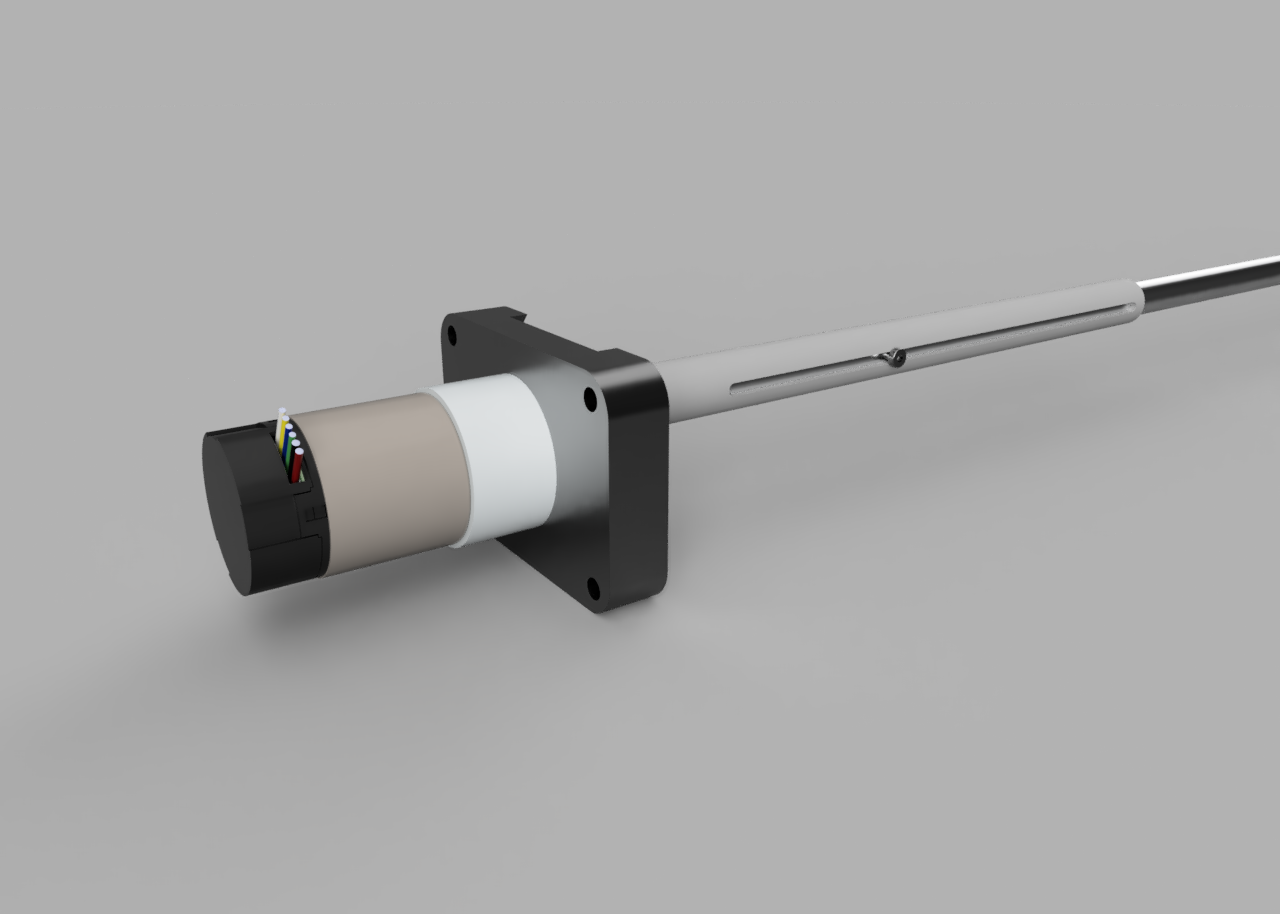
\includegraphics[width=\linewidth]{../../photos/turn_side_c}
                    \caption*{\color{hopro_darkblue}DC Motor}
                \end{center}
            \end{minipage}%
%            ~\hspace{0.1\linewidth}
            \begin{minipage}{0.5\linewidth}
                \begin{center}
                    \setcaptiontype{figure}% Fake a figure environment
                    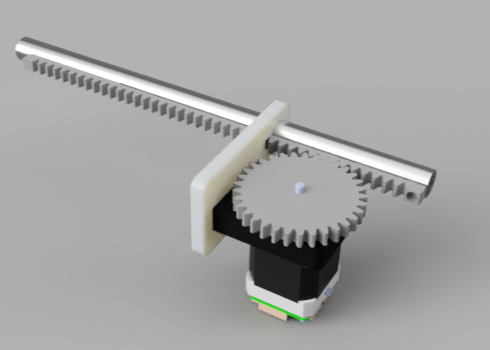
\includegraphics[width=\linewidth]{../../photos/move_side_gear_c}
                    \caption*{\color{hopro_darkblue}Stepper motor}
                \end{center}
            \end{minipage}%
        }

        \headerbox{5. Functioning of the robot goalkeeper}{name=flowchart,span=2,column=1,below=construction,above=bottom}{ % To reduce this block to 1 column width, remove 'span=2'
            The flowchart below describes the whole process of the robot detecting detecting and catching a ball.
            First, the camera records a distorted image of the table.
            This image is undistorted by the respective algorithm.
            A prerecorded image is subtracted, in order to find the ball, using a sophisticated algorithm.
            The future position is predicted by a linear regression model.
            This position and the arrival time are sent to the arduino.
            The arduino moves the goalkeeper to the predicted ball position and shoots at the correct time.
            \vspace{5pt}
            \setcaptiontype{figure}% Fake a figure environment
            \begin{center}
                \centering
                \scalebox{0.95}{
                    \begin{tikzpicture}[node distance=2cm]
%                        flowchart
                        \node (cam) [io] {Camera};
                        \node (undistortion) [process, below of=cam] {Undistortion};
                        \node (ball_detection) [process, below of=undistortion] {Ball detection};
                        \node (prediction) [process, below of=ball_detection] {Prediction};
                        \node (where) [process, below of=prediction, right of=prediction, xshift=1.5cm] {Where?};
                        \node (when) [process, below of=prediction, left of=prediction, xshift=-1.5cm] {When?};
                        \node (arduino) [process, below of=when, right of=when, xshift=1.5cm] {Arduino};
                        \node (cnc) [process, below of=arduino, right of=arduino, xshift=1.5cm] {CNC shield};
                        \node (cnc-text)  [above of=cnc, yshift=-1cm] {Target player position};
                        \node (drv) [process, below of=cnc] {DRV8825};
                        \node (stepper) [io, below of=drv] {Stepper Motor};
                        \node (stepper-text) [below of=stepper, yshift=1cm] {Move side};
                        \node (l298n) [process, below of=arduino, left of=arduino, xshift=-1.5cm] {L298N};
                        \node (shoot-text)  [above of=l298n, yshift=-1cm] {Shoot the ball};
                        \node (dc) [io, below of=l298n] {DC Motor};
                        \node (dc-text) [below of=dc, yshift=1cm] {Shoot side};

                        % arrows
                        \draw [arrow] (cam) -- (undistortion);
                        \draw [arrow] (undistortion) -- (ball_detection);
                        \draw [arrow] (ball_detection) -- (prediction);
                        \draw [arrow] (prediction) |- (where);
                        \draw [arrow] (prediction) |- (when);
                        \draw [arrow] (where) |- (arduino);
                        \draw [arrow] (when) |- (arduino);

                        \draw [arrow] (arduino) |- (cnc);
                        \draw [arrow] (cnc) -- (drv);
                        \draw [arrow] (drv) -- (stepper);
                        \draw [arrow] (arduino) |- (l298n);
                        \draw [arrow] (l298n) -- (dc);


                        \coordinate (corner1) at ([xshift=-0.3cm]when.west |- undistortion.north);


%                        photos and textboxes

%                        \node[draw, text width=5cm] at (0,-2) {}
                        \node (undistortion_original) [left of=ball_detection, xshift=-4.5cm, yshift=1cm] {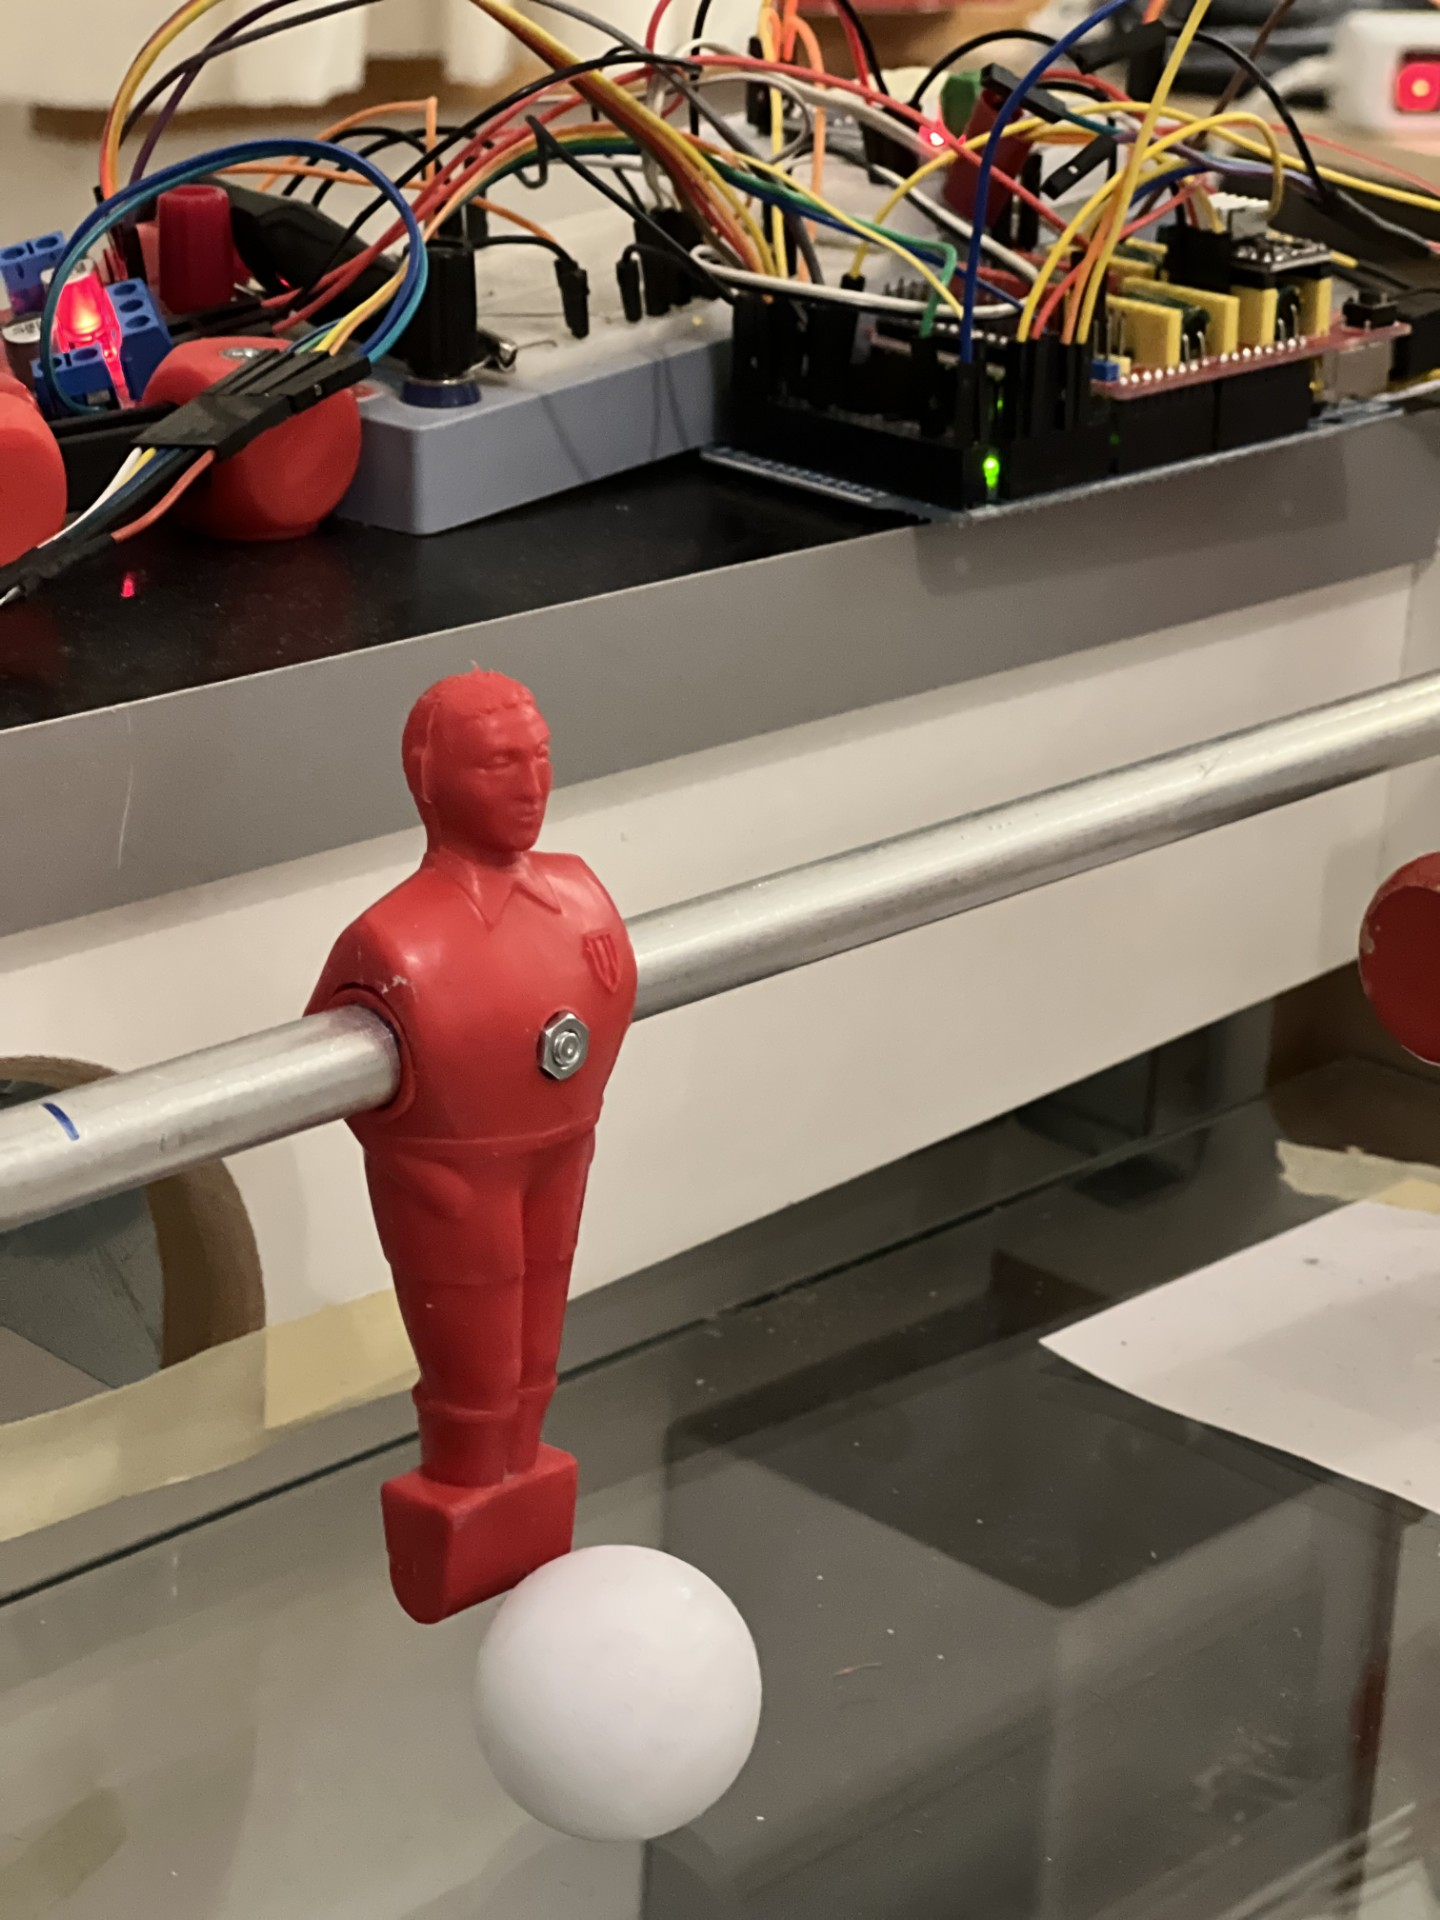
\includegraphics[width=5.5cm]{../../photos/title}};
                        \node (undistortion_undistorted) [right of=ball_detection, xshift=4.5cm, yshift=1cm] {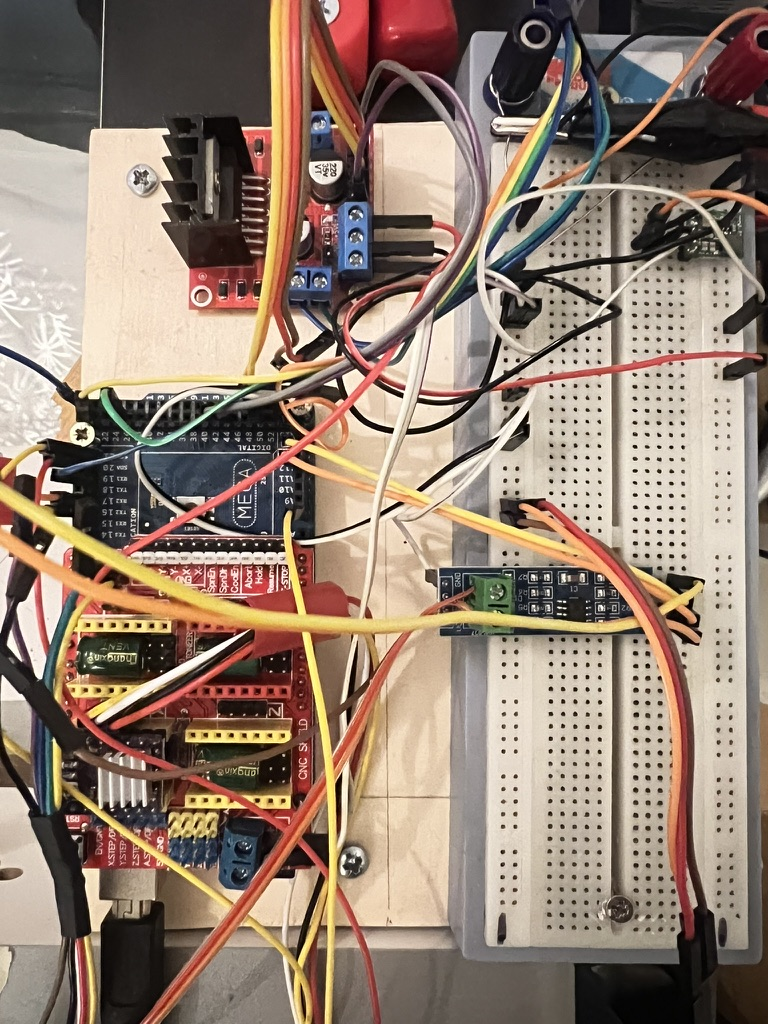
\includegraphics[width=5.5cm]{../../photos/cnc_shield_c}};

                    \end{tikzpicture}
                }
                \caption*{\color{hopro_darkblue}Flowchart for the foosball robot}
                \label{fig:whole-flowchart}
            \end{center}
        }


%        \headerbox{5. DeCAF vs. SEA}{name=sea,span=2,column=1,below=screen}{ % To reduce this block to 1 column width, remove 'span=2'
%
%            \begin{wrapfigure}{l}{0.3\textwidth}
%                \vspace{10pt}
%                \begin{center}
%                    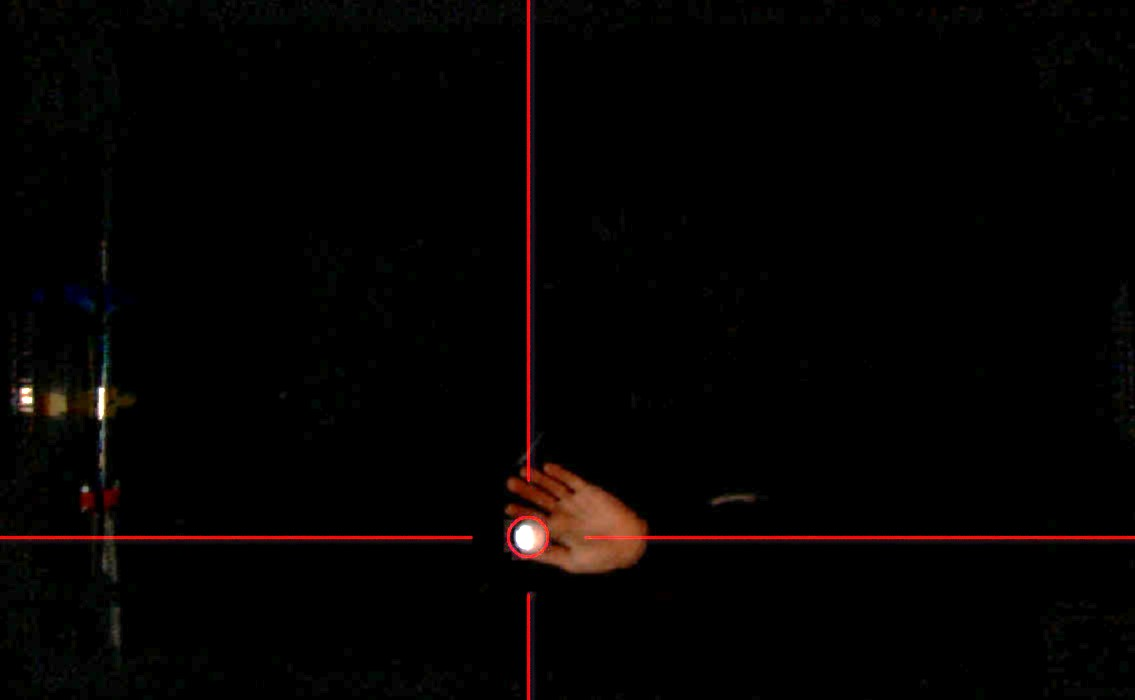
\includegraphics[width=\linewidth]{../../photos/ball_detection}
%                \end{center}
%%\vspace{-145pt}
%            \end{wrapfigure}
%
%% We tested DeCAF in 35 case studies taken from the DUD-E database, to evaluate its power to discriminate between active and inactive molecules.
%% We used DeCAF as a classifier and compared it to the SEA (Similarity Ensemble Approach) algorithm \cite{keiser2007relating}.
%% To compare sets of ligands, we adapted the approach used in SEA, replacing Tc by DCAF.
%% We prepared datasets as shown in the left diagram.
%% Then, we tested both classifiers calculating ROC AUC values for every target (below).
%            We tested DeCAF in 35 diverse targets taken from the DUD-E database, to evaluate its power to classify molecules as active or inactive.
%            We compared DeCAF to the renowned \textbf{SEA (Similarity Ensemble Approach)} algorithm \cite{keiser2007relating}, which uses Tc as a similarity measure.
%            Dataset preparation steps are shown on the left diagram.
%            Comparison results (\textbf{ROC AUC} values for each receptor) are shown below.
%% Please ask me about details.
%
%            \hspace{0pt}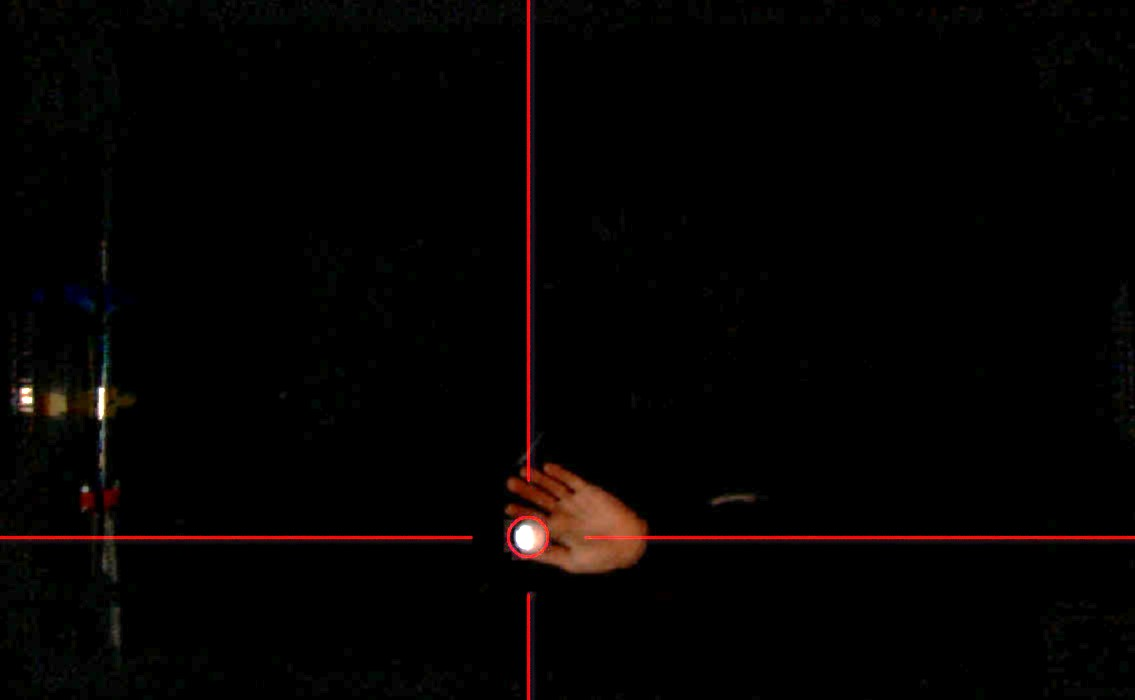
\includegraphics[width=0.95\linewidth]{../../photos/ball_detection}
%
%        }
%
%
%        \headerbox{6. Conclusions}{name=conclusion,column=1,below=sea,span=2,above=bottom}{
%% DeCAF is a chemoinformatical tool that can be helpful in ligand-based drug design.
%% It provides a comprehensive molecule description and a fast algorithms for comparing and aligning multiple ligands.
%            We proved that DeCAF is a significant improvement over the SEA algorithm, a popular method for comparing sets of ligands.
%            \begin{boenumerate}
%                \compresslist
%                \item DeCAF gives better results for 23 out of 35 receptors.
%                \item For targets with easily separable active and inactive datasets, SEA and DeCAF give similar results.
%                \item In cases in which SEA fails to identify active molecules, our method performs substantially better.
%            \end{boenumerate}
%% It can be also used in other [procedures], such as database screening or drug repositioning.
%% DeCAF is written in Python and freely available at \textbf{\color{darkgreen}http://bitbucket.org/marta-sd/decaf}.
%        }

        \headerbox{6. Results}{name=results,column=0,below=electronics,span=1}{
            This project successfully demostrates the proof of concept for a foosball goalkeeper robot.
            Slow balls are stopped reliably.
            Fast balls sometimes still cause accuracy problems.
            Unfortunately, the goalkeeper is not capable of shooting the ball back everytime.
        }


%        \headerbox{7. Acknowledgements}{name=references,column=0,span=1,below=results}{
%            \begin{itemize}
%                \setlength\itemsep{-0.1cm}
%                \item Clemens Pohle
%                \item My parents
%                \item Gabriel Schneider, Marcel Honegger, Michael Wüthrich (ZHAW)
%                \item Robert \& Ilena Teng
%            \end{itemize}
%        }

        \headerbox{7. QR Code}{name=qr_code,column=0,span=1,below=results,above=bottom}{
            \begin{center}
                Further Photos and videos can be found here:\\
                
\includegraphics[height=0.75\linewidth]{../../photos/qr_code}
            \end{center}
        }

    \end{poster}

\end{document}

